\documentclass{article}
\bibliographystyle{plainnat}
\usepackage{amsmath, amssymb}
\usepackage{url}
%\usepackage{bibentry}
\usepackage{natbib}
\usepackage{minted} % Add this to your preamble for beautiful Python code formatting
%\usepackage{listings} % Add this line for code formatting
%\lstset{language=Python, basicstyle=\small\ttfamily, breaklines=true} % Basic Python style
%\usepackage[breaklines]{minted}
\usepackage{graphicx}
\usepackage{enumitem}
\usepackage{titlesec}

\usepackage[margin=1in]{geometry}



\title{The Illustrated GRPO: A Detailed and Pedagogical Explanation of GRPO Algorithm}
%\author{Abderrahman Skiredj}

\author{
  {\Large Abderrahman Skiredj} \\
  \vspace{0.2em}
  {\small OCP Solutions \& College of Computing, Mohammed VI Polytechnic University, Morocco} \\
  {\small \texttt{abderrahman.skiredj@um6p.ma}}
}

\date{April 2025}

\begin{document}

\maketitle

\section*{Introduction}

Adapting large language models (LLMs) to specific tasks often involves prompting, Retrieval-Augmented Generation (RAG), or agentic systems. Prompting suits quick, general tasks but falters in complex reasoning or specialization. RAG excels with external knowledge but struggles to teach new skills or control output style. Agentic systems fit dynamic goals yet can overcomplicate simpler needs. Group Relative Policy Optimization (GRPO), a DeepSeek reinforcement learning method, is ideal when deep domain expertise, precise style and tone control, specific output formatting, or debiasing are required—particularly for reasoning-intensive tasks without clear answers, as shown in DeepSeekMath. This paper offers a clear, comprehensive guide to GRPO, blending theory, math, and practical steps. Where existing resources scatter or omit details, we provide a unified, pedagogical resource to unlock GRPO’s potential for fine-tuning LLMs effectively.

The paper is organized into \textbf{four main sections} to provide a comprehensive understanding of GRPO from theory to practice. The first section offers a \textbf{theoretical deep dive}, detailing the algorithm’s mechanics with rigor and intuitive explanations. The second section serves as a \textbf{practical tutorial}, guiding readers through a quick application of GRPO using the TRL library with simplified steps and examples. The third section presents \textbf{a simplified, didactic implementation of GRPO}, designed for clarity and educational purposes, using a small model and basic prompts. Finally, the fourth section explores an optimized, \textbf{industrial-grade implementation from the TRL library}, mapping theoretical steps to production-ready code.


\section{GRPO algorithm: Deep dive}
\label{sec:grpo_deep_dive}
\textbf{Overview of the GRPO Algorithm} \\
Group Relative Policy Optimization (GRPO) fine-tunes a language model by iteratively improving its policy through group-based reward comparisons. The algorithm proceeds as follows:
\begin{enumerate}
    \item Sample \( G \) outputs per query from a batch using the current policy \( \pi_{\theta_{\text{old}}} \).
    \item Evaluate each output with a reward model to assign scalar rewards \( r_i \).
    \item Compute advantages \( A_i \) by normalizing rewards relative to the group’s mean and standard deviation.
    \item Calculate a surrogate loss using clipped probability ratios between the current policy \( \pi_\theta \) and old policy, with a KL penalty for stability.
    \item Update the policy parameters \( \theta \) via backpropagation to maximize expected rewards.
\end{enumerate}
These steps are illustrated in Figure~\ref{grpo_diagram}, which applies them to fine-tune an LLM on mathematical reasoning.

Let us now delve into the details of each step.\\
\vspace{3mm}

\begin{figure}[h]
    \centering
    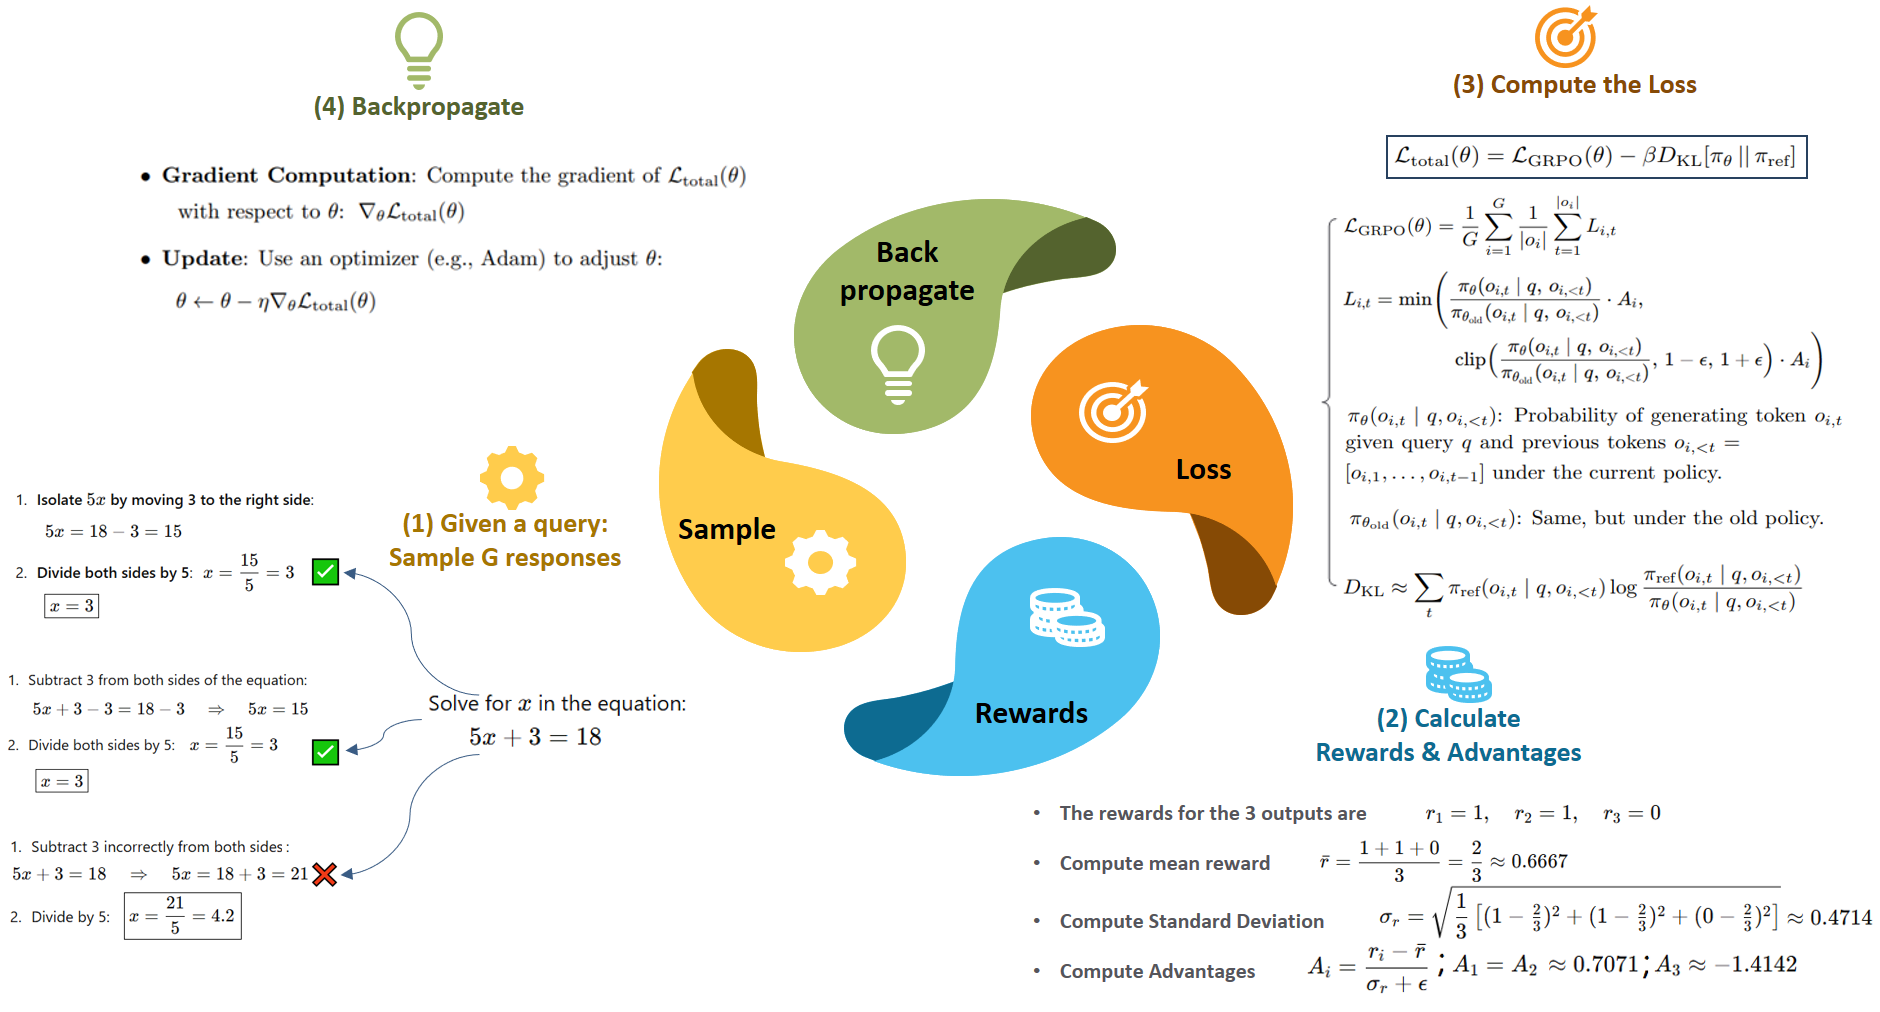
\includegraphics[width=1.05\linewidth]{my_diagram2.png}
    \caption{Overview of the GRPO algorithm workflow.}
    \label{grpo_diagram}
\end{figure}

\noindent\textbf{Step 1: Prepare a Batch of Training Queries} \\
Take a batch of training queries \( \{q_1, q_2, \dots, q_B\} \), where \( B \) is the batch size. These are questions or prompts the model will respond to.\\

\vspace{3mm}

\noindent\textbf{Step 2: Sample \( G \) Outputs for a Single Query} \\
For simplicity, consider a single query \( q \) from the batch. Using the current policy model with parameters \( \theta_{\text{old}} \) (denoted \( \pi_{\theta_{\text{old}}} \)), generate \( G \) different outputs \( \{o_1, o_2, \dots, o_G\} \). Each output \( o_i \) is a sequence of tokens 
\[
o_i = [o_{i,1}, o_{i,2}, \dots, o_{i,|o_i|}],
\]
where \( |o_i| \) is the length of the sequence.\\[1mm]
Why \( G \) Outputs?: Sampling multiple outputs allows GRPO to compare them relative to each other, forming a group-based baseline for rewards.

\vspace{3mm}

\noindent\textbf{Step 3: Calculate Rewards and Advantages}
\begin{itemize}
    \item \textbf{Reward Assignment}: Pass each output \( o_i \) to a reward model, which assigns a scalar reward \( r_i \) based on quality (e.g., accuracy, coherence). You get 
\[
\{r_1, r_2, \dots, r_G\}.
\]


To make this more concrete, DeepSeek uses a rule-based strategy tailored to each task, such as math or coding. The reward \( r_i \) for an output \( o_i \) is computed using a weighted combination:
\[
r_i = \alpha \cdot \text{accuracy\_score} + \beta \cdot \text{format\_score},
\]
where \( \alpha \) and \( \beta \) are task-specific weights balancing correctness and structure.

For the accuracy score, math tasks use regular expressions to extract the final answer and compare it to the ground truth (1 if correct, 0 otherwise). Coding tasks run the code in a sandbox and assign a score based on how many test cases pass. The format score, on the other hand, checks whether the output follows the expected structure—such as including reasoning within specific tags like \texttt{<think>}—and is typically binary (1 if well-structured, 0 if not).
    \item \textbf{Compute Statistics}:
    \begin{itemize}
        \item Mean reward: \( \bar{r} = \frac{1}{G} \sum_{i=1}^{G} r_i \)
        \item Standard deviation of rewards: \( \sigma_r = \sqrt{\frac{1}{G} \sum_{i=1}^{G} (r_i - \bar{r})^2} \)
    \end{itemize}
    \item \textbf{Compute Advantage}: For each output \( o_i \), the advantage is:
\[
A_i = \frac{r_i - \bar{r}}{\sigma_r + \epsilon}
\]
\textbf{Terms}:
\begin{itemize}
    \item \( r_i \): Reward for output \( o_i \).
    \item \( \bar{r} \): Mean reward across the \( G \) outputs.
    \item \( \sigma_r \): Standard deviation of rewards (measures variability).
    \item \( \epsilon \): Small constant (e.g., \( 10^{-8} \)) to avoid division by zero if \( \sigma_r = 0 \).
\end{itemize}
The idea is that by normalizing the reward relative to the group, indicating how much better or worse \( o_i \) is compared to the average, the model learns to favor responses with \( A_i > 0 \) and suppress those with \( A_i < 0 \). For instance, if \( A_i = 0.94 \), the model increases the likelihood of generating that (correct) response.\\[1mm]
Note that in standard GRPO (outcome supervision), the advantage \( A_i \) is the same for all tokens \( o_{i,t} \) in output \( o_i \). So, \( A_{i,t} = A_i \) for all \( t = 1, 2, \dots, |o_i| \). This is because the reward \( r_i \) is given for the entire output \( o_i \), not per token or step.\\[1mm]
\textbf{Exception}: In process supervision (not standard GRPO), rewards are given per reasoning step, and advantages could vary per token or segment. But for this explanation, we assume outcome supervision, so \( A_{i,t} = A_i \).
\end{itemize}

\vspace{3mm}

\noindent\textbf{Step 4: Compute the Surrogate Loss} 
\begin{itemize}
    \item \textbf{Probability Ratio}: For each token \( o_{i,t} \) in output \( o_i \), compute the ratio of probabilities between the current policy \( \pi_\theta \) and the old policy \( \pi_{\theta_{\text{old}}} \):
\[
\text{ratio}_{i,t} = \frac{\pi_\theta(o_{i,t} \mid q, o_{i,<t})}{\pi_{\theta_{\text{old}}}(o_{i,t} \mid q, o_{i,<t})}
\]
\textbf{Terms}:
\begin{itemize}
    \item \( \pi_\theta(o_{i,t} \mid q, o_{i,<t}) \): Probability of generating token \( o_{i,t} \) given query \( q \) and previous tokens \( o_{i,<t} = [o_{i,1}, \dots, o_{i,t-1}] \) under the current policy.
    \item \( \pi_{\theta_{\text{old}}}(o_{i,t} \mid q, o_{i,<t}) \): Same, but under the old policy.
\end{itemize}
The idea is to measure how much the policy has changed for that token.
    \item \textbf{Clipped Objective} Define the clipped term:
\[
g(\epsilon, A_i) = \text{clip}(\text{ratio}_{i,t}, 1 - \epsilon, 1 + \epsilon) \cdot A_i
\]
\textbf{Terms}:
\begin{itemize}
    \item \( \text{clip}(x, a, b) \): Clamps \( x \) between \( a \) and \( b \) (i.e., \( \max(a, \min(b, x)) \)).
    \item \( \epsilon \): Hyperparameter (e.g., 0.2) controlling the clipping range.
    \item \( A_i \): Advantage for output \( o_i \).
\end{itemize}
The idea is to limit large policy updates for stability.
\item \textbf{Loss per Token}: For each token \( o_{i,t} \):
\[
L_{i,t} = \min \left( \text{ratio}_{i,t} \cdot A_i, \; g(\epsilon, A_i) \right)
\]
\textbf{Terms}:
\begin{itemize}
    \item \( \text{ratio}_{i,t} \cdot A_i \): Unclipped objective (encourages policy to favor high-advantage outputs).
    \item \( g(\epsilon, A_i) \): Clipped objective (caps the update size).
\end{itemize}
The idea is to take the minimum to conservatively update the policy: The clipping restricts the policy update ratio to \([1 - \epsilon, 1 + \epsilon]\) to avoid large shifts from the old policy. This in particular limits overconfident updates.

Example with \(\epsilon = 0.2\): if \(\pi_{\theta}(o_i|q) = 0.9\), \(\pi_{\text{old}}(o_i|q) = 0.5\), then ratio \(= 1.8 \rightarrow\) clip to 1.2. If new policy gives 0.2, then \(0.2 / 0.5 = 0.4 \rightarrow\) clip to 0.8.



\item \textbf{Total Surrogate Loss}: Average over all tokens and outputs:
\[
\mathcal{L}_{\text{GRPO}}(\theta) = \frac{1}{G} \sum_{i=1}^{G} \frac{1}{|o_i|} \sum_{t=1}^{|o_i|} L_{i,t}
\]
\textbf{Terms}:
\begin{itemize}
    \item \( \frac{1}{G} \): Normalizes across the \( G \) outputs.
    \item \( \frac{1}{|o_i|} \): Normalizes across the length of each output \( o_i \).
    \item \( L_{i,t} \): Loss contribution from each token.
\end{itemize}
\item \textbf{KL Divergence Penalty}: Add a penalty to prevent large deviations from a reference policy \( \pi_{\text{ref}} \) (e.g., initial policy):
\[
\mathcal{L}_{\text{total}}(\theta) = \mathcal{L}_{\text{GRPO}}(\theta) - \beta D_{\text{KL}}[\pi_\theta \,||\, \pi_{\text{ref}}]
\]
\textbf{Terms}:
\begin{itemize}
    \item \( D_{\text{KL}}[\pi_\theta \,||\, \pi_{\text{ref}}] \): KL divergence, approximated per token as:
    \[
    D_{\text{KL}} \approx \sum_{t} \pi_{\text{ref}}(o_{i,t} \mid q, o_{i,<t}) \log \frac{\pi_{\text{ref}}(o_{i,t} \mid q, o_{i,<t})}{\pi_\theta(o_{i,t} \mid q, o_{i,<t})}
    \]
    \item \( \beta \): Hyperparameter (e.g., 0.01) controlling penalty strength.
\end{itemize}
The idea is to ensure stability by keeping \( \pi_\theta \) close to \( \pi_{\text{ref}} \). A KL divergence penalty keeps the model’s outputs near the original distribution, preventing extreme shifts while still allowing controlled exploration and refinement.

The $\beta$ parameter controls the strength of the KL divergence penalty. A higher $\beta$ keeps the policy close to the reference, ensuring stability but slowing exploration. A lower $\beta$ allows faster adaptation and more deviation, but risks instability or reward hacking. The original DeepSeekMath paper used $\beta= 0.04$.

\end{itemize}





\vspace{3mm}

\noindent\textbf{Step 5: Backpropagate and Update the Policy} \\
\begin{itemize}
    \item \textbf{Gradient Computation}: Compute the gradient of \( \mathcal{L}_{\text{total}}(\theta) \) with respect to \( \theta \):
\[
\nabla_\theta \mathcal{L}_{\text{total}}(\theta)
\]
\item \textbf{Update}: Use an optimizer (e.g., Adam) to adjust \( \theta \):
\[
\theta \leftarrow \theta - \eta \nabla_\theta \mathcal{L}_{\text{total}}(\theta)
\]
\textbf{Terms}:
\begin{itemize}
    \item \( \eta \): Learning rate (e.g., \( 10^{-5} \)).
\end{itemize}
The idea is to minimize the loss, effectively maximizing the expected reward by adjusting token probabilities.
\end{itemize}




\noindent\textbf{Summary of Key Formulas}
\begin{enumerate}
    \item \textbf{Advantage}: \( A_i = \frac{r_i - \bar{r}}{\sigma_r + \epsilon} \), uniform for all tokens in \( o_i \).
    \item \textbf{Probability Ratio}: \( \text{ratio}_{i,t} = \frac{\pi_\theta(o_{i,t} \mid q, o_{i,<t})}{\pi_{\theta_{\text{old}}}(o_{i,t} \mid q, o_{i,<t})} \).
    \item \textbf{Clipped Term}: \( g(\epsilon, A_i) = \text{clip}(\text{ratio}_{i,t}, 1 - \epsilon, 1 + \epsilon) \cdot A_i \).
    \item \textbf{Token Loss}: \( L_{i,t} = \min \left( \text{ratio}_{i,t} \cdot A_i, \; g(\epsilon, A_i) \right) \).
    \item \textbf{Total Loss}: \( \mathcal{L}_{\text{total}}(\theta) = \frac{1}{G} \sum_{i=1}^{G} \frac{1}{|o_i|} \sum_{t=1}^{|o_i|} L_{i,t} - \beta D_{\text{KL}}[\pi_\theta \,||\, \pi_{\text{ref}}] \).
\end{enumerate}

\noindent\textbf{Limitations \& Challenges of GRPO}:
The following passage is taken directly from the HuggingFace Reasoning Course \citep{reasoning_course}:
\begin{itemize}
    \item Generation Cost: Generating multiple completions (4-16) for each prompt increases computational requirements compared to methods that generate only one or two completions.
\item Batch Size Constraints: The need to process groups of completions together can limit effective batch sizes, adding complexity to the training process and potentially slowing down training.
\item Reward Function Design: The quality of training heavily depends on well-designed reward functions. Poorly designed rewards can lead to unintended behaviors or optimization for the wrong objectives.
\item Group Size Tradeoffs: Choosing the optimal group size involves balancing diversity of solutions against computational cost. Too few samples may not provide enough diversity, while too many increase training time and resource requirements.
\item KL Divergence Tuning: Finding the right balance for the KL divergence penalty requires careful tuning: too high and the model won’t learn effectively, too low and it may diverge too far from its initial capabilities.
\end{itemize}

\section{Practical Tutorial Using TRL Library}
\label{sec:tutorial}

In addition to the theoretical aspects described above, we draw inspiration from the excellent practical tutorial available online \citep{huggingface_unsloth_colab}. It makes use of the TRL implementation of the GRPO Algorithm \citep{trl}. Here, we simplify the content to focus on the most important components.


\subsection*{Data Preparation}

The tutorial uses the GSM8K dataset, a collection of math word problems designed to test reasoning skills. Each entry consists of a question and an answer, with the final numerical solution typically marked by \texttt{\#\#\#\#} in the answer text. 

\vspace{0.5em}
\noindent To give a clearer picture, here are two sample entries from the dataset:\\
\textbf{Sample 1:}
\begin{itemize}
    \item \textbf{Question}: Kawtar sold clips to 48 of her friends in April, and then she sold half as many clips in May. How many clips did Kawtar sell altogether in April and May?
    \item \textbf{Answer}: Kawtar sold 48/2 = 24 clips in May. Kawtar sold 48+24 = 72 clips altogether in April and May. \texttt{\#\#\#\# 72}
\end{itemize}
\textbf{Sample 2:}
\begin{itemize}
\item \textbf{Question}: Weng earns \$12 an hour for babysitting. Yesterday, she just did 50 minutes of babysitting. How much did she earn?
\item \textbf{Answer}: Weng earns 12/60 = \$0.2 per minute. Working 50 minutes, she earned 0.2 $\times$ 50 = \$10. \texttt{\#\#\#\# 10}
\end{itemize}
\vspace{0.5em}


\vspace{0.5em}
The first step is to extract the final answer (e.g., ``72'' or ``10'') for evaluation. We define a function to do this:

\begin{minted}[fontsize=\small, bgcolor=gray!5, frame=lines, framesep=2mm, baselinestretch=1.1, linenos]{python}
def extract_hash_answer(text):
    if "####" not in text:
        return None
    return text.split("####")[1].strip()
\end{minted}

For instance, applying this to Sample 1’s answer yields ``72''. 

\vspace{0.5em}
Next, we define a system prompt to guide the model’s output format, encouraging it to show its reasoning and provide a solution within specific tags:

\begin{minted}[fontsize=\small, bgcolor=gray!5, frame=lines, framesep=2mm, baselinestretch=1.1, linenos]{python}
reasoning_start = "<start_working_out>"
reasoning_end   = "<end_working_out>"
solution_start  = "<SOLUTION>"
solution_end    = "</SOLUTION>"

system_prompt = f"""You are given a problem.
Think about the problem and provide your working out.
Place it between {reasoning_start} and {reasoning_end}.
Then, provide your solution between {solution_start}{solution_end}"""
\end{minted}

The dataset is then mapped to pair each question with this system prompt and the extracted answer, preparing it for GRPO training.

\subsection*{Reward Functions}

Reward functions are the heart of GRPO, as they evaluate the quality of the model’s outputs and drive policy optimization. 

\vspace{0.5em}
The tutorial defines multiple reward functions, but we highlight two key examples here for clarity.

\vspace{0.5em}
The first, \texttt{match\_format\_exactly}, awards points if the output adheres precisely to the expected structure, including both reasoning and solution sections:

\begin{minted}[fontsize=\small, bgcolor=gray!5, frame=lines, framesep=2mm, baselinestretch=1.1, linenos]{python}
def match_format_exactly(completions, **kwargs):
    scores = []
    for completion in completions:
        score = 0
        response = completion[0]["content"]
        if match_format.search(response) is not None:
            score += 3.0
        scores.append(score)
    return scores
\end{minted}

Here, \texttt{match\_format} is a regular expression ensuring the presence of all required tags in the correct order (defined earlier in the code, omitted here for brevity). An output like:

\begin{center}
  \texttt{<start\_working\_out>Let’s think!<end\_working\_out><SOLUTION>42</SOLUTION>}
\end{center}

would score 3.0, while a malformed response would score 0.

\vspace{0.5em}
The second function, \texttt{check\_answer}, evaluates the correctness of the solution by comparing the extracted answer to the ground truth:

\begin{minted}[fontsize=\small, bgcolor=gray!5, frame=lines, framesep=2mm, baselinestretch=1.1, linenos]{python}
def check_answer(prompts, completions, answer, **kwargs):
    scores = []
    for completion, true_answer in zip(completions, answer):
        score = 0
        response = completion[0]["content"]
        guess = match_format.search(response).group(1) if match_format.search(response) else None
        if guess == true_answer:
            score += 3.0
        elif guess.strip() == true_answer.strip():
            score += 1.5
        scores.append(score)
    return scores
\end{minted}

This function awards 3.0 for an exact match (e.g., ``72'' vs. ``72''), 1.5 for a match ignoring whitespace, and 0 otherwise. Additional reward functions (e.g., partial format matching or numerical closeness) enhance flexibility.

\subsection*{Training with GRPO}

Training is performed using the \texttt{GRPOTrainer} from the TRL library~\cite{trl}. The Gemma3 model, enhanced with LoRA adapters via Unsloth for efficient fine-tuning, is trained on the prepared dataset with the defined reward functions. Key hyperparameters are set as follows:

\begin{minted}[fontsize=\small, bgcolor=gray!5, frame=lines, framesep=2mm, baselinestretch=1.1, linenos]{python}
from trl import GRPOConfig, GRPOTrainer

training_args = GRPOConfig(
    learning_rate=5e-6,
    per_device_train_batch_size=1,
    num_generations=4,  # Number of outputs G per query
    max_steps=50,
    max_prompt_length=256,
    max_completion_length=768,
    output_dir="outputs",
)

trainer = GRPOTrainer(
    model=model,
    processing_class=tokenizer,
    reward_funcs=[match_format_exactly, check_answer],
    args=training_args,
    train_dataset=dataset,
)

trainer.train()
\end{minted}

Here, \texttt{num\_generations=4} corresponds to \( G \) in our theoretical explanation, generating four outputs per query to compute group-based advantages.\\

Some \textbf{Practical tips} include:
\begin{itemize}
    \item \textbf{num\_generation}: Defines group size in GRPO (completions per prompt); 2-3 lacks diversity, 4-16 balances efficiency and variety, larger boosts learning but costs more—adjust based on resources and task complexity
    \item \textbf{Memory}: Tune \texttt{per\_device\_train\_batch\_size} and \texttt{gradient\_accumulation\_steps} to fit GPU memory; enable \texttt{use\_vllm=True} for faster generation if supported
    \item \textbf{Monitoring}: Track training metrics—\texttt{reward} (average across completions), \texttt{reward\_std} (variation within groups), and \texttt{kl} (divergence from reference model)
\end{itemize}

\vspace{1em}
This concludes the preparation and training procedure, where reward-guided optimization plays a central role in refining the model’s ability to reason and answer accurately.

%\section{Deep Dive into the TRL implementation of the GRPO Algorithm}

\section{Simple \& Didactical Implementation of the GRPO Algorithm}

In this section, we present a simplified yet functional implementation of the GRPO (Generalized Reward Policy Optimization) algorithm, fully taken from the HuggingFace Reasoning Course \citep{reasoning_course}, but rearranged for improved pedagogical clarity. It bridges the theoretical framework outlined in Section~\ref{sec:grpo_deep_dive} with concrete code, using the small model \texttt{Qwen/Qwen2-Math-1.5B} and a basic math prompt for focus and accessibility.
In the subsequent section, we explore the optimized, industrial-grade implementation of GRPO provided by HuggingFace's TRL library, illustrating how the same algorithm scales to production-ready use cases.


\subsection*{Loading the Model and Generating Responses}

This stage corresponds to \textbf{Step 1} and \textbf{Step 2} of the theoretical overview. We load a pre-trained language model and generate multiple responses for a batch of prompts.

We use two prompts:
\begin{itemize}
  \item \( q_1 \): "Solve \( y = 2x + 1 \) for \( x = 2 \), \( y = \)" (correct answer: 5)
  \item \( q_2 \): "Solve \( y = 2x + 1 \) for \( x = 4 \), \( y = \)" (correct answer: 9)
\end{itemize}

Here, the batch size \( B = 2 \) (two queries), and we generate \( G = 4 \) responses per query, totaling 8 responses.

\begin{minted}[fontsize=\small, bgcolor=gray!5, frame=lines, framesep=2mm, baselinestretch=1.1, linenos]{python}
import torch
from transformers import AutoModelForCausalLM, AutoTokenizer

# Load the model and tokenizer
model_name = "Qwen/Qwen2-Math-1.5B"
model = AutoModelForCausalLM.from_pretrained(model_name)
tokenizer = AutoTokenizer.from_pretrained(model_name)
model.eval()

# Move model to GPU if available
device = torch.device("cuda" if torch.cuda.is_available() else "cpu")
model.to(device)

# Input prompts (batch of 2 queries)
prompts = [
    "Solve y = 2x + 1 for x = 2, y = ",  # Correct answer: 5
    "Solve y = 2x + 1 for x = 4, y = "   # Correct answer: 9
]
inputs = tokenizer(prompts, return_tensors="pt", padding=True)
input_ids = inputs["input_ids"].to(device)  # Shape: (2, prompt_len)
attention_mask = inputs["attention_mask"].to(device)

# Generate 4 responses per prompt (B=2, G=4, total 8 responses)
batch_size = len(prompts)  # 2
num_generations = 4
outputs = model.generate(
    input_ids=input_ids,  # Shape: (2, prompt_len)
    attention_mask=attention_mask,
    max_new_tokens=1,  # Single-token response
    num_return_sequences=num_generations,  # 4 per prompt
    do_sample=True,
    top_k=10,
    temperature=0.7,
    pad_token_id=tokenizer.eos_token_id,
    return_dict_in_generate=True,
    output_scores=True,
)
\end{minted}

\textbf{Comments:}
\begin{itemize}
  \item \textbf{Model Loading:} We load \texttt{Qwen/Qwen2-Math-1.5B} and its tokenizer, representing the current policy \( \pi_{\theta_{\text{old}}} \) (Step 1). The model is set to evaluation mode and moved to the GPU if available.
  \item \textbf{Prompt Preparation:} We define a batch of \( B = 2 \) prompts, tokenized into \texttt{input\_ids} with shape \( (2, \text{prompt\_len}) \), matching Step 1’s batch of queries \( \{q_1, q_2\} \).
  \item \textbf{Response Generation:} The \texttt{model.generate} call produces \( G = 4 \) responses per prompt. With \texttt{input\_ids} of shape \( (2, \text{prompt\_len}) \) and \texttt{num\_return\_sequences=4}, it generates \( 2 \times 4 = 8 \) total responses (Step 2). The \texttt{max\_new\_tokens=1} ensures single-token outputs (e.g., "5", "9"). Sampling parameters (\texttt{top\_k=10}, \texttt{temperature=0.7}) ensure diversity. Example output:
  \begin{itemize}
    \item \( q_1 \): [5, 6, 7, 5]
    \item \( q_2 \): [10, 2, 9, 9]
  \end{itemize}
\end{itemize}

\subsection*{Calculating Rewards and Advantages}

This stage implements \textbf{Step 3}: assigning rewards, computing group-wise statistics, and calculating advantages.

For the generated responses:
\begin{itemize}
  \item \( q_1 \) (correct answer: 5): [5, 6, 7, 5]
  \item \( q_2 \) (correct answer: 9): [10, 2, 9, 9]
\end{itemize}

We use a binary reward: \( r_i = 1 \) if correct, \( 0 \) otherwise:
\begin{itemize}
  \item \( q_1 \) rewards: [1, 0, 0, 1]
  \item \( q_2 \) rewards: [0, 0, 1, 1]
\end{itemize}

\begin{minted}[fontsize=\small, bgcolor=gray!5, frame=lines, framesep=2mm, baselinestretch=1.1, linenos]{python}
# Rewards for the 8 responses (flattened)
rewards = torch.tensor([1, 0, 0, 1, 0, 0, 1, 1], dtype=torch.float32)  # Shape: (8,)
# Note: In practice, rewards are computed by comparing generated tokens to correct answers (5, 9)

# Group rewards: Shape (B, G) = (2, 4)
rewards_grouped = rewards.view(batch_size, num_generations)

# Mean per group: Shape (B,) = (2,)
mean_grouped_rewards = rewards_grouped.mean(dim=1)

# Std per group: Shape (B,) = (2,)
std_grouped_rewards = rewards_grouped.std(dim=1)

# Broadcast to match rewards: Shape (8,)
mean_grouped_rewards = mean_grouped_rewards.repeat_interleave(num_generations)
std_grouped_rewards = std_grouped_rewards.repeat_interleave(num_generations)

# Advantages: Shape (8,)
advantages = (rewards - mean_grouped_rewards) / (std_grouped_rewards + 1e-8)

# Reshape to match logits: Shape (8, 1)
advantages = advantages.unsqueeze(1)
\end{minted}

\textbf{Explanation:}
\begin{itemize}
  \item \textbf{Reward Assignment:} Rewards are assigned per query: \( q_1 \) (answer: 5) gets [1, 0, 0, 1]; \( q_2 \) (answer: 9) gets [0, 0, 1, 1]. In practice, we’d decode the generated tokens and compare them to the correct answers (Step 3).
  \item \textbf{Grouping:} \texttt{rewards\_grouped} becomes \( (2, 4) \):
  \[
  \begin{bmatrix} 1 & 0 & 0 & 1 \\ 0 & 0 & 1 & 1 \end{bmatrix}
  \]
  \item \textbf{Statistics:} Mean: [0.5, 0.5], Std: [0.5774, 0.5774]
  \item \textbf{Broadcasting:} Mean and std are repeated: [0.5, 0.5, 0.5, 0.5, 0.5, 0.5, 0.5, 0.5]
  \item \textbf{Advantages:} \( A_i = \frac{r_i - \bar{r}}{\sigma_r + 10^{-8}} \), e.g., \( A_1 = \frac{1 - 0.5}{0.5774} \approx 0.8659 \), yielding [0.8659, -0.8660, -0.8660, 0.8659, -0.8660, -0.8660, 0.8659, 0.8659]
\end{itemize}

\subsection*{Updating the Policy}

This stage implements \textbf{Step 4} (surrogate loss) and \textbf{Step 5} (policy update), using advantages to refine the model.

\begin{minted}[fontsize=\small, bgcolor=gray!5, frame=lines, framesep=2mm, baselinestretch=1.1, linenos]{python}
import torch.nn.functional as F

# Assume log probs are available (Shape: (8, 1))
# In practice, computed by passing outputs through old and new models
per_token_logps = ...  # Old policy log probs
new_per_token_logps = ...  # New policy log probs

# Probability ratio: Shape (8, 1)
ratio = torch.exp(new_per_token_logps - per_token_logps)

# Clipping
eps = 0.2
pg_losses1 = -advantages * ratio
pg_losses2 = -advantages * torch.clamp(ratio, 1.0 - eps, 1.0 + eps)
pg_loss_max = torch.max(pg_losses1, pg_losses2)

# KL penalty: Shape (8, 1)
per_token_kl = F.kl_div(
    F.log_softmax(new_per_token_logps, dim=-1),
    F.softmax(per_token_logps, dim=-1),
    reduction="none",
).sum(dim=-1, keepdim=True)

# Total loss
beta = 0.01
per_token_loss = pg_loss_max + beta * per_token_kl
total_loss = per_token_loss.mean()

# Update model
optimizer = torch.optim.Adam(model.parameters(), lr=1e-5)
optimizer.zero_grad()
total_loss.backward()
optimizer.step()
\end{minted}

\textbf{Explanation:}
\begin{itemize}
  \item \textbf{Ratio:} \( \frac{\pi_\theta}{\pi_{\theta_{\text{old}}}} \) guides the policy shift (Step 4).
  \item \textbf{Clipped Loss:} Combines unclipped and clipped terms, stabilized with \( \epsilon = 0.2 \).
  \item \textbf{KL Penalty:} Regularizes with \( \beta = 0.01 \).
  \item \textbf{Update:} Adam optimizes \( \theta \) to maximize rewards (Step 5).
\end{itemize}




\section{Deep Dive into the TRL Implementation of the GRPO Algorithm}

In this section, we explore how the GRPO algorithm is implemented in the TRL library’s \texttt{GRPOTrainer} class. The difference between the previous section is that the following code is an optimized and industrial-grade implementation of GRPO provided by HuggingFace's TRL library.
Each step outlined in Section 1 is meticulously mapped to specific methods and code segments, providing a clear bridge between theory and practice. We use the code from the TRL library (version as of April 2025).

\subsection*{Step 1: Prepare a Batch of Training Queries}

\textbf{What It Does in Theory}: The first step involves preparing a batch of training queries \( \{q_1, q_2, \dots, q_B\} \), where \( B \) is the batch size. These queries serve as the prompts that the model will respond to, forming the foundation for subsequent steps.

\textbf{Implementation in TRL}: In the \texttt{GRPOTrainer} class, this step is handled by the data loading mechanism inherited from the \texttt{Trainer} class in the \texttt{transformers} library, customized with a special sampler. The \texttt{\_get\_train\_sampler} method defines a \texttt{RepeatRandomSampler} that prepares batches in a unique way:

\begin{minted}[fontsize=\small, bgcolor=gray!5, frame=lines, framesep=2mm, baselinestretch=1.1, linenos]{python}
def _get_train_sampler(self) -> Sampler:
    effective_batch_size = (
        self.args.per_device_train_batch_size
        * self.accelerator.num_processes
        * self.args.gradient_accumulation_steps
    )
    return RepeatRandomSampler(
        data_source=self.train_dataset,
        mini_repeat_count=self.num_generations,
        batch_size=effective_batch_size // self.num_generations,
        repeat_count=self.num_iterations,
        seed=self.args.seed,
    )
\end{minted}

\begin{itemize}
    \item \textbf{Dataset Source}: The \texttt{train\_dataset} contains the prompts (stored under the key \texttt{"prompt"}).
    
    \item \textbf{Custom Sampling}: The \texttt{RepeatRandomSampler} repeats each prompt \texttt{num\_generations} times (denoted \( G \) in the theory) within each batch. This ensures that for every unique prompt \( q_i \), there are \( G \) instances in the batch, allowing the generation of multiple outputs later.
    
    \item \textbf{Batch Size}: The \texttt{effective\_batch\_size} accounts for the number of devices and gradient accumulation steps, ensuring scalability across distributed setups. The number of unique prompts per batch is \( \text{effective\_batch\_size} / G \).
    
    \item \textbf{Repetition Across Updates}: The \texttt{repeat\_count=self.num\_iterations} parameter allows the same batch to be reused across multiple optimization steps, a feature unique to GRPO for efficiency.
\end{itemize}

This setup guarantees that the batch is structured to support the generation of \( G \) outputs per query, aligning with Step 2. The sampler’s design also ensures consistency across processes in distributed training, which is crucial for reward normalization later.

\subsection*{Step 2: Sample \( G \) Outputs for a Single Query}

\textbf{What It Does in Theory}: For each query \( q \) in the batch, the current policy \( \pi_{\theta_{\text{old}}} \) generates \( G \) different outputs \( \{o_1, o_2, \dots, o_G\} \), where each \( o_i \) is a sequence of tokens.

\textbf{Implementation in TRL}: This step occurs in the \texttt{\_generate\_and\_score\_completions} method, called within \texttt{\_prepare\_inputs} during training:

\begin{minted}[fontsize=\small, bgcolor=gray!5, frame=lines, framesep=2mm, baselinestretch=1.1, linenos, breaklines]{python}
def _prepare_inputs(self, inputs: dict[str, Union[torch.Tensor, Any]]) -> dict[str, Union[torch.Tensor, Any]]:
    mode = "eval" if self.control.should_evaluate else "train"
    if mode == "train":
        buffer_index = self._step % self.args.gradient_accumulation_steps
        buffered_inputs = self._buffered_inputs[buffer_index]
        if self.state.global_step % self.num_iterations == 0 or buffered_inputs is None:
            inputs = self._generate_and_score_completions(inputs)
            self._buffered_inputs[buffer_index] = inputs
        else:
            inputs = buffered_inputs
        self._step += 1
    else:
        inputs = self._generate_and_score_completions(inputs)
    return inputs
\end{minted}

Inside \texttt{\_generate\_and\_score\_completions}:

\begin{minted}[fontsize=\small, bgcolor=gray!5, frame=lines, framesep=2mm, baselinestretch=1.1, linenos, breaklines]{python}
prompts = [x["prompt"] for x in inputs]
prompts_text = [maybe_apply_chat_template(example, self.processing_class)["prompt"] for example in inputs]
prompt_inputs = self.processing_class(
    text=prompts_text, return_tensors="pt", padding=True, padding_side="left", add_special_tokens=False
)
prompt_inputs = super()._prepare_inputs(prompt_inputs)
prompt_ids, prompt_mask = prompt_inputs["input_ids"], prompt_inputs["attention_mask"]

if self.args.use_vllm:
    all_prompts_text = gather_object(prompts_text)
    if self.accelerator.is_main_process:
        ordered_set_of_prompts = all_prompts_text[:: self.num_generations]
        with profiling_context(self, "vLLM.generate"):
            completion_ids = self.vllm_client.generate(
                prompts=ordered_set_of_prompts,
                n=self.num_generations,
                max_tokens=self.max_completion_length,
                # ... other sampling parameters ...
            )
    completion_ids = broadcast_object_list(completion_ids, from_process=0)
    process_slice = slice(
        self.accelerator.process_index * len(prompts),
        (self.accelerator.process_index + 1) * len(prompts),
    )
    completion_ids = completion_ids[process_slice]
    completion_ids = [torch.tensor(ids, device=device) for ids in completion_ids]
    completion_ids = pad(completion_ids, padding_value=self.processing_class.pad_token_id)
    prompt_completion_ids = torch.cat([prompt_ids, completion_ids], dim=1)
else:
    with unwrap_model_for_generation(self.model_wrapped, self.accelerator) as unwrapped_model:
        prompt_completion_ids = unwrapped_model.generate(
            prompt_ids, attention_mask=prompt_mask, generation_config=self.generation_config
        )
    prompt_length = prompt_ids.size(1)
    completion_ids = prompt_completion_ids[:, prompt_length:]
\end{minted}

\begin{itemize}
    \item \textbf{Prompt Preparation}: The prompts are extracted from the batch and tokenized into \texttt{prompt\_ids}.
    
    \item \textbf{Generation Paths}:
    \begin{itemize}
        \item \textbf{With vLLM}: If \texttt{use\_vllm} is enabled, the main process generates \( G \) completions per unique prompt using the vLLM client. Since the batch has duplicates (from the sampler), it takes unique prompts and generates \texttt{num\_generations} outputs, which are then distributed to all processes.
        
        \item \textbf{Without vLLM}: The model’s \texttt{generate} method produces one completion per prompt instance. Because the sampler repeats each prompt \( G \) times, this results in \( G \) outputs per unique prompt across the batch.
    \end{itemize}
    
    \item \textbf{Output Format}: The completions are stored as \texttt{completion\_ids}, concatenated with \texttt{prompt\_ids} for later processing.
\end{itemize}

\textbf{Key Detail}: The \texttt{num\_generations} parameter directly corresponds to \( G \), controlling how many outputs are sampled per query, fulfilling the theoretical requirement.

\subsection*{Step 3: Calculate Rewards and Advantages}

\textbf{What It Does in Theory}: Each output \( o_i \) is evaluated by a reward model to obtain rewards \( \{r_1, r_2, \dots, r_G\} \). The mean \( \bar{r} \) and standard deviation \( \sigma_r \) are computed, and the advantage for each output is calculated as \( A_i = \frac{r_i - \bar{r}}{\sigma_r + \epsilon} \).

\textbf{Implementation in TRL}: This is also handled in \texttt{\_generate\_and\_score\_completions}:

\begin{minted}[fontsize=\small, bgcolor=gray!5, frame=lines, framesep=2mm, baselinestretch=1.1, linenos, breaklines]{python}
rewards_per_func = torch.zeros(len(prompts), len(self.reward_funcs), device=device)
for i, (reward_func, reward_processing_class) in enumerate(
    zip(self.reward_funcs, self.reward_processing_classes)
):
    if isinstance(reward_func, nn.Module):
        texts = [p + c for p, c in zip(prompts, completions)]
        reward_inputs = reward_processing_class(
            text=texts, return_tensors="pt", padding=True, padding_side="right", add_special_tokens=False
        )
        reward_inputs = super()._prepare_inputs(reward_inputs)
        with torch.inference_mode():
            rewards_per_func[:, i] = reward_func(**reward_inputs).logits[:, 0]
    else:
        reward_kwargs = {key: [example[key] for example in inputs] for key in inputs[0] if key != "prompt"}
        output_reward_func = reward_func(prompts=prompts, completions=completions, **reward_kwargs)
        output_reward_func = [r if r is not None else torch.nan for r in output_reward_func]
        rewards_per_func[:, i] = torch.tensor(output_reward_func, dtype=torch.float32, device=device)

rewards = (rewards_per_func * self.reward_weights.to(device).unsqueeze(0)).nansum(dim=1)

mean_grouped_rewards = rewards.view(-1, self.num_generations).mean(dim=1)
std_grouped_rewards = rewards.view(-1, self.num_generations).std(dim=1)

advantages = rewards - mean_grouped_rewards.repeat_interleave(self.num_generations, dim=0)
if self.args.scale_rewards:
    advantages = advantages / (std_grouped_rewards.repeat_interleave(self.num_generations, dim=0) + 1e-4)
\end{minted}

\begin{itemize}
    \item \textbf{Reward Computation}: For each completion, rewards are calculated using multiple \texttt{reward\_funcs} (e.g., models or custom functions). The total reward \( r_i \) is a weighted sum of individual rewards, matching the theoretical \( r_i = \alpha \cdot \text{accuracy\_score} + \beta \cdot \text{format\_score} \).
    
    \item \textbf{Grouping}: Rewards are reshaped into groups of size \( G \) (\texttt{self.num\_generations}) to compute per-group statistics.
    
    \item \textbf{Advantages}: The advantage \( A_i \) is computed as \( r_i - \bar{r} \), and if \texttt{scale\_rewards} is True, it’s normalized to \( \frac{r_i - \bar{r}}{\sigma_r + 10^{-4}} \), directly implementing the formula from Step 3.
\end{itemize}


The group-based normalization is a hallmark of GRPO, enabling relative comparisons within each query’s outputs.

\subsection*{Step 4: Compute the Surrogate Loss}

\textbf{What It Does in Theory}: This step computes the probability ratio \( \text{ratio}_{i,t} = \frac{\pi_\theta(o_{i,t} \mid q, o_{i,<t})}{\pi_{\theta_{\text{old}}}(o_{i,t} \mid q, o_{i,<t})} \), the clipped term \( g(\epsilon, A_i) \), and the per-token loss \( L_{i,t} = \min(\text{ratio}_{i,t} \cdot A_i, g(\epsilon, A_i)) \). The total loss includes a KL penalty: \( \mathcal{L}_{\text{total}}(\theta) = \frac{1}{G} \sum_{i=1}^{G} \frac{1}{|o_i|} \sum_{t=1}^{|o_i|} L_{i,t} - \beta D_{\text{KL}}[\pi_\theta \,||\, \pi_{\text{ref}}] \).

\vspace{2mm}

\noindent \textbf{Implementation in TRL}: This is implemented in the \texttt{compute\_loss} method:

\begin{minted}[fontsize=\small, bgcolor=gray!5, frame=lines, framesep=2mm, baselinestretch=1.1, linenos, breaklines]{python}
@profiling_decorator
def compute_loss(self, model, inputs, return_outputs=False, num_items_in_batch=None):
    prompt_ids, prompt_mask = inputs["prompt_ids"], inputs["prompt_mask"]
    completion_ids, completion_mask = inputs["completion_ids"], inputs["completion_mask"]
    input_ids = torch.cat([prompt_ids, completion_ids], dim=1)
    attention_mask = torch.cat([prompt_mask, completion_mask], dim=1)
    logits_to_keep = completion_ids.size(1)

    per_token_logps = self._get_per_token_logps(model, input_ids, attention_mask, logits_to_keep)

    if self.beta != 0.0:
        ref_per_token_logps = inputs["ref_per_token_logps"]
        per_token_kl = (
            torch.exp(ref_per_token_logps - per_token_logps) - (ref_per_token_logps - per_token_logps) - 1
        )

    advantages = inputs["advantages"]
    old_per_token_logps = inputs["old_per_token_logps"] if self.num_iterations > 1 else per_token_logps.detach()
    coef_1 = torch.exp(per_token_logps - old_per_token_logps)
    coef_2 = torch.clamp(coef_1, 1 - self.epsilon_low, 1 + self.epsilon_high)
    per_token_loss1 = coef_1 * advantages.unsqueeze(1)
    per_token_loss2 = coef_2 * advantages.unsqueeze(1)
    per_token_loss = -torch.min(per_token_loss1, per_token_loss2)
    if self.beta != 0.0:
        per_token_loss = per_token_loss + self.beta * per_token_kl
    loss = (per_token_loss * completion_mask).sum() / completion_mask.sum()
    return loss
\end{minted}

\begin{minted}[fontsize=\small, linenos, breaklines]{python}
def _get_per_token_logps(self, model, input_ids, attention_mask, logits_to_keep):
    # We add 1 to `logits_to_keep` because the last logits of the sequence is later excluded
    logits = model(input_ids=input_ids, attention_mask=attention_mask, logits_to_keep=logits_to_keep + 1).logits
    logits = logits[:, :-1, :]  # (B, L-1, V), exclude the last logit: it corresponds to the next token pred

    input_ids = input_ids[:, -logits_to_keep:]
    # For transformers<=4.48, logits_to_keep argument isn't supported, so here we drop logits ourselves.
    # See https://github.com/huggingface/trl/issues/2770
    logits = logits[:, -logits_to_keep:]
    # Divide logits by sampling temperature.
    # compute logprobs for the input tokens
\end{minted}

\begin{itemize}
    \item \textbf{Log Probabilities}: The \texttt{\_get\_per\_token\_logps} method computes per-token log probabilities for the current model (\texttt{per\_token\_logps}) and, if needed, the reference model (\texttt{ref\_per\_token\_logps}).
    
    \item \textbf{Probability Ratio}:
    \begin{itemize}
        \item \( \text{ratio}_{i,t} \) is calculated as \( \exp(\text{per\_token\_logps} - \text{old\_per\_token\_logps}) \), stored in \texttt{coef\_1}. This is the exponential of the log probability difference, equivalent to \( \frac{\pi_\theta(o_{i,t})}{\pi_{\theta_{\text{old}}}(o_{i,t})} \).
    \end{itemize}
    
    \item \textbf{Clipped Term}:
    \begin{itemize}
        \item \( g(\epsilon, A_i) \) is implemented as\\
        \texttt{coef\_2 = torch.clamp(coef\_1, 1 - self.epsilon\_low, 1 + self.epsilon\_high)} multiplied by \texttt{advantages}, ensuring the ratio stays within \( [1 - \epsilon, 1 + \epsilon] \).
    \end{itemize}
    
    \item \textbf{Per-Token Loss}:
    \begin{itemize}
        \item \texttt{per\_token\_loss1 = coef\_1 * advantages} is the unclipped term.
        \item \texttt{per\_token\_loss2 = coef\_2 * advantages} is the clipped term.
        \item \texttt{per\_token\_loss = -torch.min(per\_token\_loss1, per\_token\_loss2)} computes \( L_{i,t} \), negated because the training loop minimizes the loss, while GRPO aims to maximize the surrogate objective.
    \end{itemize}
    
    \item \textbf{KL Penalty}: If \texttt{beta != 0}, the KL term is approximated as \( \exp(\text{ref\_logps} - \text{logps}) - (\text{ref\_logps} - \text{logps}) - 1 \), added to the loss scaled by \texttt{beta}.
    
    \item \textbf{Total Loss}: The final \texttt{loss} averages \( L_{i,t} \) over all tokens, masked by \texttt{completion\_mask}, matching \( \frac{1}{G} \sum_{i=1}^{G} \frac{1}{|o_i|} \sum_{t=1}^{|o_i|} L_{i,t} \).
\end{itemize}

\textbf{Why the Negative Sign?}: In RL, we maximize the surrogate objective, but the \texttt{Trainer} minimizes the loss. Thus, \( L_{i,t} \) is negated to align with this convention.

\textbf{Key Detail}: The KL penalty uses an approximation rather than the exact \( D_{\text{KL}} \), which simplifies computation and is effective for small policy changes.
The KL divergence penalty \( \beta D_{\text{KL}}[\pi_\theta \,||\, \pi_{\text{ref}}] \) is approximated per token as \( \exp(x) - x - 1 \), where \( x = \log \frac{\pi_{\text{ref}}(o_{i,t})}{\pi_\theta(o_{i,t})} \). For small policy updates, this expands to \( \frac{1}{2} x^2 + \mathcal{O}(x^3) \), mirroring the second-order behavior of the KL divergence for the chosen token \( o_{i,t} \). This approximation avoids summing over the full vocabulary, balancing computational efficiency with effective regularization in GRPO.

\subsection*{Step 5: Backpropagate and Update the Policy}

\textbf{What It Does in Theory}: Compute the gradient \( \nabla_\theta \mathcal{L}_{\text{total}}(\theta) \) and update the policy parameters using an optimizer: \( \theta \leftarrow \theta - \eta \nabla_\theta \mathcal{L}_{\text{total}}(\theta) \).

\textbf{Implementation in TRL}: This step leverages the \texttt{Trainer} class’s training loop, with no explicit override in \texttt{GRPOTrainer} for the update itself:

\begin{itemize}
    \item \textbf{Loss Computation}: The \texttt{compute\_loss} method returns the loss, as shown above.
    
    \item \textbf{Training Loop}: In the \texttt{Trainer.train} method (inherited from \texttt{transformers}), the following occurs:
    \begin{enumerate}
        \item \textbf{Forward Pass}: Calls \texttt{compute\_loss} to get the loss.
        \item \textbf{Backward Pass}: Executes \texttt{loss.backward()} to compute gradients.
        \item \textbf{Optimization}: The optimizer (e.g., Adam, configured via \texttt{optimizers} in \texttt{\_\_init\_\_}) updates the parameters using the learning rate \( \eta \) (e.g., \texttt{learning\_rate=5e-6} from your tutorial).
    \end{enumerate}
\end{itemize}


\textbf{Code Context}: While not explicitly shown in \texttt{GRPOTrainer}, the inherited training step can be conceptualized as:

\begin{minted}[fontsize=\small, bgcolor=gray!5, frame=lines, framesep=2mm, baselinestretch=1.1, linenos]{python}
# From transformers.Trainer.train (simplified)
for step, inputs in enumerate(epoch_iterator):
    inputs = self._prepare_inputs(inputs)
    loss = self.compute_loss(model, inputs)
    loss = loss / self.args.gradient_accumulation_steps
    loss.backward()
    if (step + 1) % self.args.gradient_accumulation_steps == 0:
        self.optimizer.step()
        self.optimizer.zero_grad()
\end{minted}

\begin{itemize}
    \item \textbf{Gradient Accumulation}: If \texttt{gradient\_accumulation\_steps > 1}, the loss is scaled and gradients are accumulated before the update, enhancing efficiency.
    
    \item \textbf{Parameter Update}: The optimizer applies \( \theta \leftarrow \theta - \eta \nabla_\theta \mathcal{L}_{\text{total}} \), where \( \eta \) is set in \texttt{GRPOConfig}.
\end{itemize}

This step finalizes the policy improvement, adjusting token probabilities to favor higher-reward outputs while maintaining stability via clipping and KL regularization.

\subsection*{Summary of the Mapping}

Here’s a concise mapping of all steps to the \texttt{GRPOTrainer} code:
\begin{enumerate}
    \item \textbf{Step 1}: \texttt{\_get\_train\_sampler} prepares batches with repeated prompts.
    \item \textbf{Step 2}: \texttt{\_generate\_and\_score\_completions} samples \( G \) outputs per query.
    \item \textbf{Step 3}: \texttt{\_generate\_and\_score\_completions} computes rewards and advantages.
    \item \textbf{Step 4}: \texttt{compute\_loss} calculates the surrogate loss with clipping and KL penalty.
    \item \textbf{Step 5}: Inherited \texttt{Trainer} training loop backpropagates the loss and updates the policy.
\end{enumerate}

\section{Conclusion}
GRPO empowers large language models with specialized skills, controlled outputs, and enhanced reasoning, surpassing traditional fine-tuning by optimizing multiple responses via a reward model. This paper delivers a concise yet thorough exploration of GRPO, from theoretical steps to practical implementation in tools like TRL. No single prior work combines its theory, practice, and nitty-gritty details—leaving gaps we now fill. By clarifying how GRPO achieves deep expertise, style precision, and debiasing, this guide equips readers to apply it confidently, advancing LLM performance for tailored, impactful use cases.
\begin{thebibliography}{9}

\bibitem{trl}
HuggingFace. \textit{GRPO Trainer in TRL Library}. Available at: \url{https://github.com/huggingface/trl/blob/main/trl/trainer/grpo_trainer.py}. Accessed: April 1, 2025.

\bibitem{huggingface_unsloth_colab}
HuggingFace and UnslothAI. \textit{Colab: HuggingFace Course - Gemma3 (1B) - GRPO}. Available at: \url{https://colab.research.google.com/github/unslothai/notebooks/blob/main/nb/HuggingFace%20Course-Gemma3_(1B)-GRPO.ipynb}. Accessed: April 1, 2025.

\bibitem{deepseekai2025deepseekr1incentivizingreasoningcapability}
DeepSeek-AI et al. (2025). \textit{DeepSeek-R1: Incentivizing Reasoning Capability in LLMs via Reinforcement Learning}. arXiv:2501.12948.

\bibitem{deepseekai2025deepseekv3technicalreport}
DeepSeek-AI et al. (2025). \textit{DeepSeek-V3 Technical Report}. arXiv:2412.19437.

\bibitem{reasoning_course}
Hugging Face, \textit{Understanding the DeepSeek R1 Paper}, Open R1 for Students. Available at: \url{https://huggingface.co/learn/nlp-course/chapter12/3?fw=pt} (Accessed: April 2, 2025).



\end{thebibliography}


\end{document}
